% !TeX root = ..\rapport_13_1.tex
\section{Kravspecifikation}
\subsection{Indledning}
Denne del af eksamensopgaven dokumenterer vores planlægningsproces, der skal tilvejebringe et tids/projektstyringsprogram der møder Softwarehuset A/S' ønsker. Det gøres ved hjælp af ideer og modeller fra Behavior- og Test Driven Development, der ved hjælp af brainstorming lader os gå fra kundeønsker til scenarier, fra scenarier til tests og fra tests til kode (tests og kode i næste rapport), alt sammen med rod i beskrivelsen af Softwarehusets ønsker.
\subsection{Ordliste}
\begin{table}[H]
    \centering
    \setlength{\extrarowheight}{8pt}
    \begin{tabular}{>{\bfseries}l p{0.73\textwidth}}
        Medarbejder           & \textit{[Employee]} En medarbejder er en person ansat i Softwarehuset A/S, som er tildelt aktiviteter. En medarbejder kan udføre aktiviteter og registrere arbejdstid brugt på aktiviteter, uagtet om medarbejderen er tilknyttet aktiviteten. Hver medarbejder har et medarbejder ID.                                     \\
        Projekt aktivitet     & \textit{[Project activity]} En delopgave af et projekt. Hver aktivitet er tilknyttet en medarbejder.                                                                                                                                                                                                                       \\
        Fast aktivitet        & \textit{[Regular activity]} Aktivitet der ikke kan pålægges et projekt. F.eks. ferie, sygdom, kurser.                                                                                                                                                                                                                      \\
        Projekt               & \textit{[Project]} Udviklingsarbejde udført for en kunde (eksternt) eller for Softwarehuset A/S (internt). Et projekt administreres af en projektleder og er inddelt i aktiviteter. Hvert projekt har et projektnummer.                                                                                                    \\
        Kunde                 & \textit{[Customer]} En ekstern entitet som bestiller og er modtager af projekter.                                                                                                                                                                                                                                          \\
        Projektleder          & \textit{[Project leader]} En medarbejder der har ret til at oprette og tildele aktiviteter for et givent projekt.                                                                                                                                                                                                          \\
        Softwarehuset A/S     & \textit{[Softwarehuset A/S]} Entitet som er modtager af et projekt, hvis projektet er internt.                                                                                                                                                                                                                             \\
        Medarbejder initialer & \textit{[Employee initials]} Unik identifikation for hver enkelt medarbejder, bestående af fire bogstaver. To første fra fornavn efterfulgt af to første fra efternavn. F.eks. rawi. Hvis initialer allerede er taget, vælges bogstav et og tre i efternavn, derefter et og fire, osv.                                     \\
        Projektnummer         & \textit{[Project number]} Identifikation for hvert enkelt projekt. Har formen årstal efterfulgt af et fireciffret løbenummer. F.eks. 23001                                                                                                                                                                                 \\
        Budgetteret tid       & \textit{[Time budget]} En aktivitets estimerede antal hele timer.                                                                                                                                                                                                                                                          \\
        Arbejdstid            & \textit{[Work time]} Mængde tid i inkrementer af halve timer, brugt på en aktivitet. Kan registreres af den medarbejder som har brugt arbejdstid på en given aktivitet.                                                                                                                                                    \\
        Start- og sluttid     & \textit{[start- and end week]} En periode med opløsning på uge-niveau til aktiviteter. Begge tider angives som år og uge, ved formatet ÅÅUU. F.eks. 2304 for uge 4 i 2023. En starttid afgrænser starten af en given uge, en sluttid afgrænser ved slutningen af en given uge. Start- og sluttid kan derfor godt være ens.
    \end{tabular}
\end{table}
\subsection{Use case diagrammer}
\begin{figure}[H]
    \centering
    \caption{Use case diagram for programmet \textbf{Timeregistrering og projektstyring} hvori de tre aktører inkluderet er Gæst, Medarbejder og Projektleder.}\label{fig:AlleActorsPaaEnGang}
    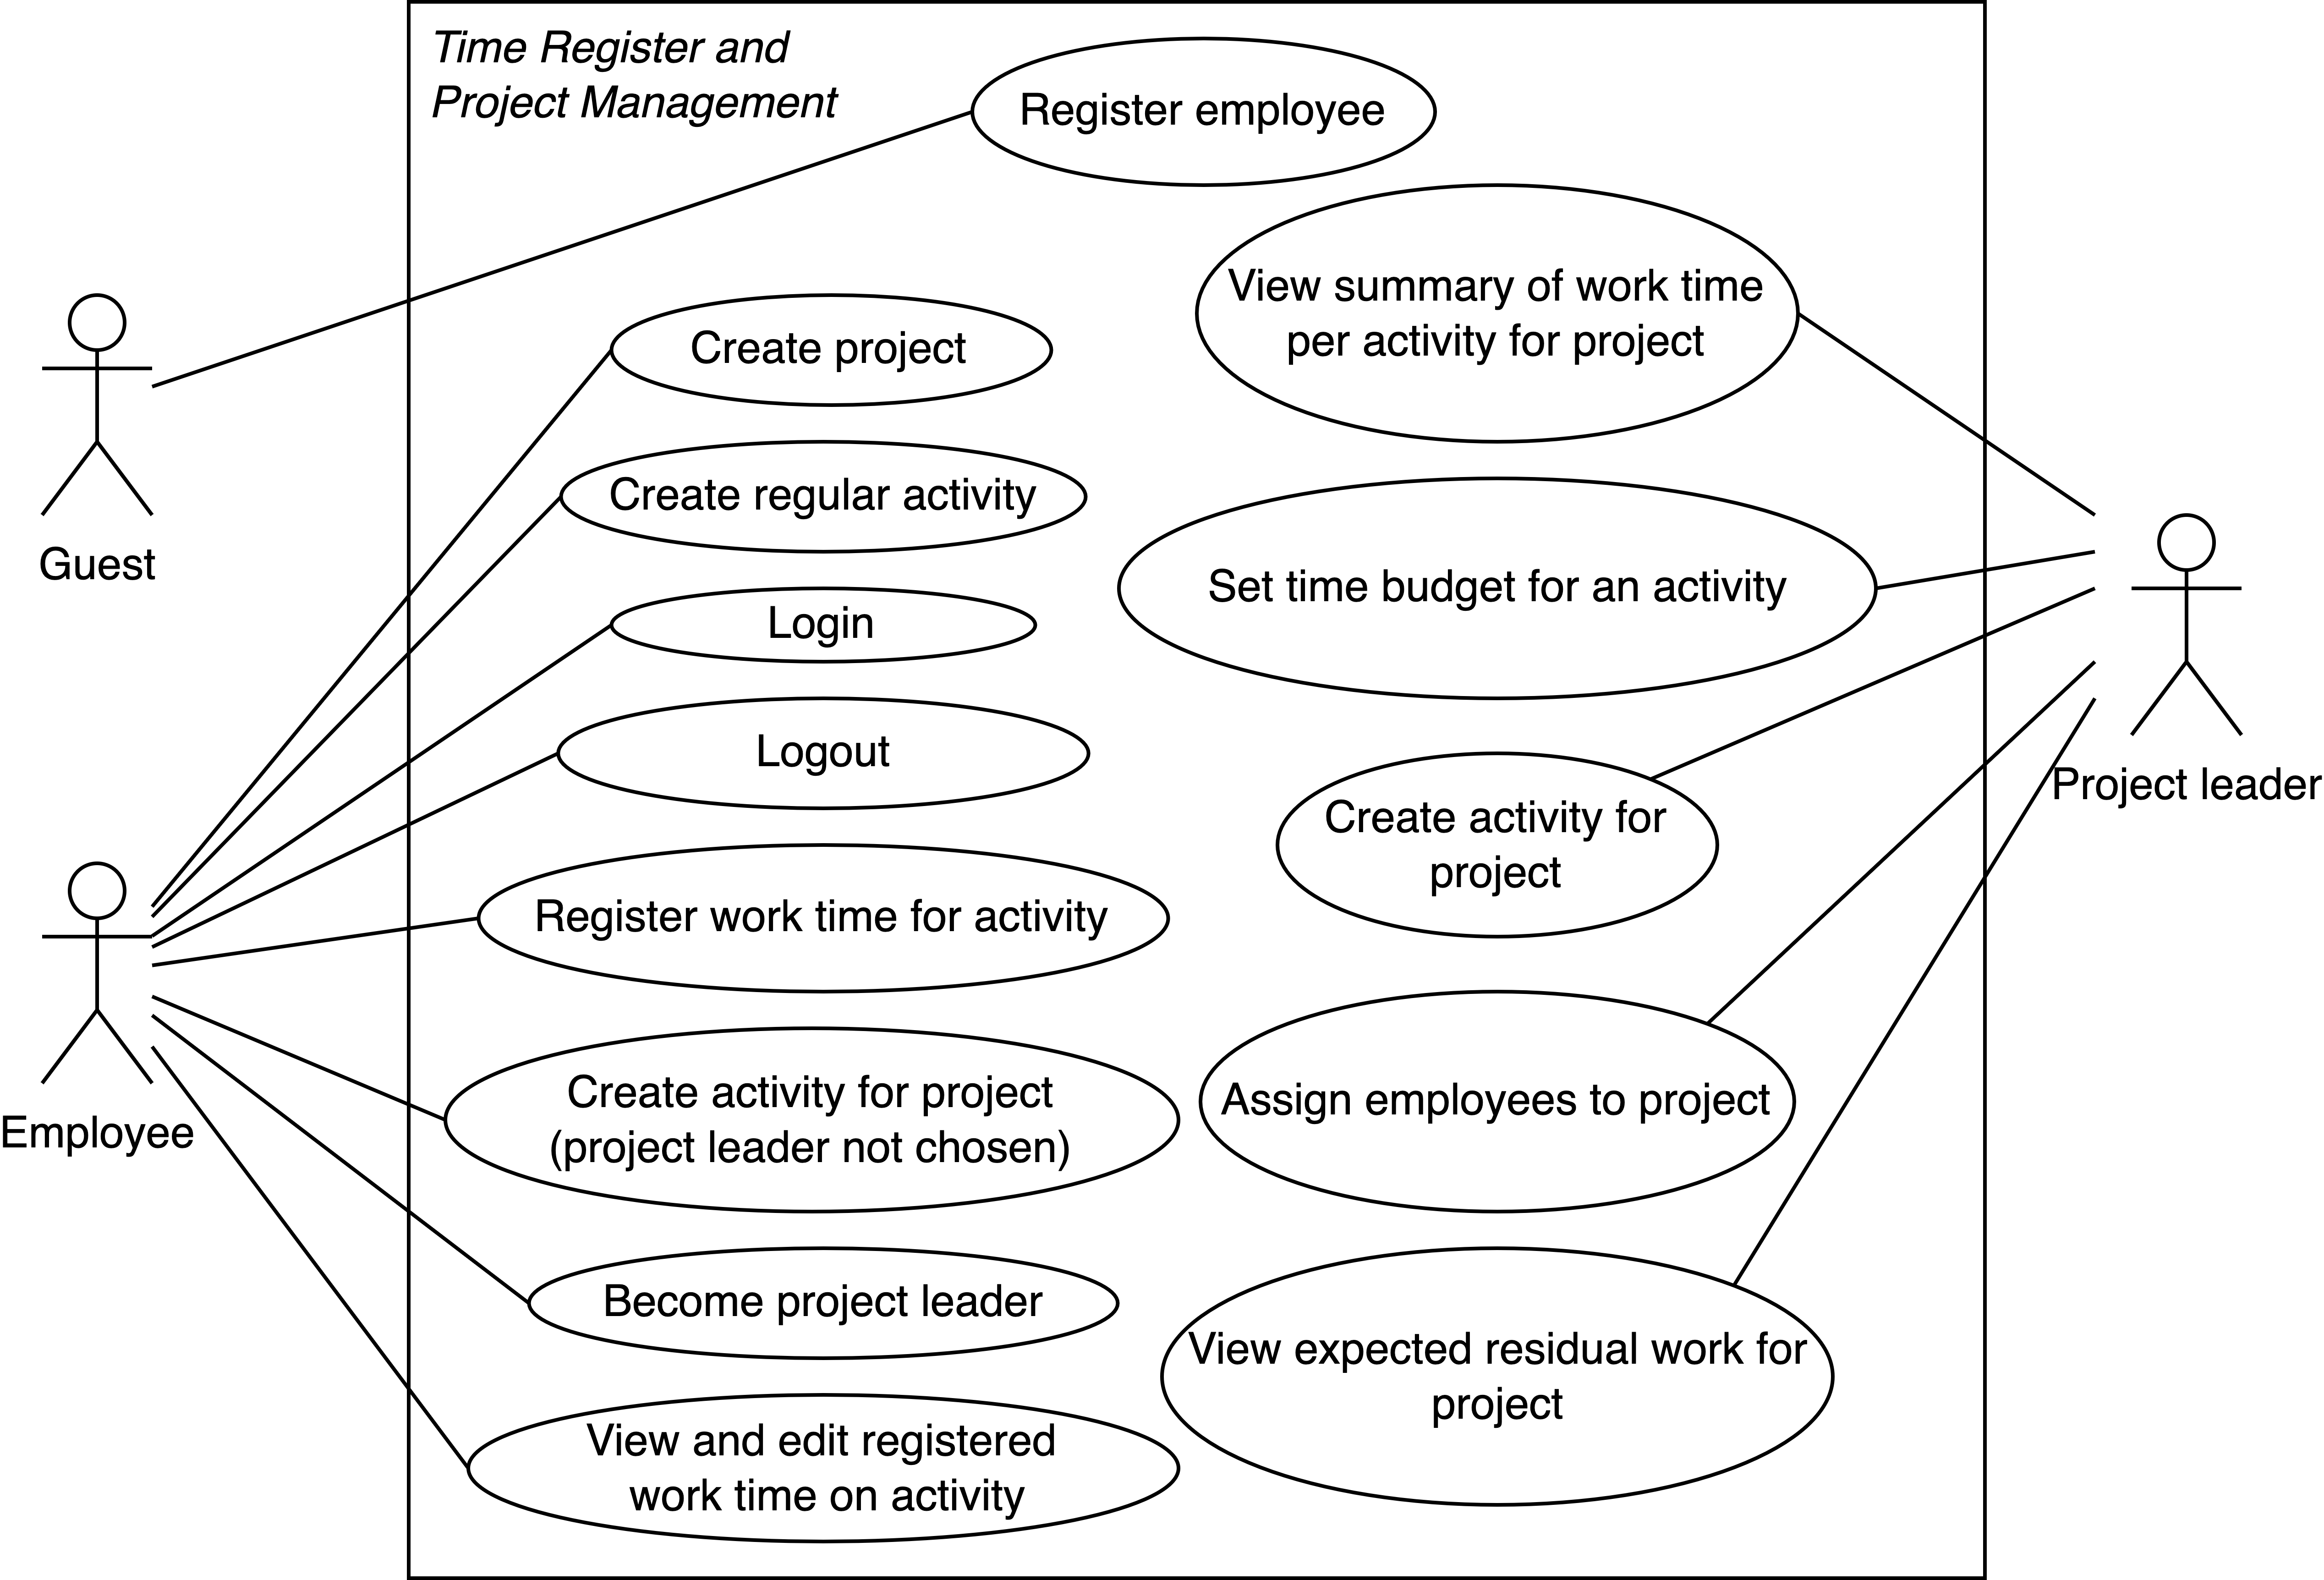
\includegraphics[width=.85\textwidth]{Diagrams/Timeregistrering og projektstyring.png}
\end{figure}
\begin{table}[H]
    \centering
    \caption{Todo usecases}
    \begin{tabular}{ll}
        Detaljeret use case                                            & Cucumber feature                                                                       \\
        \midrule
        Opret Medarbejder                                              & \cref{lst:usecase_register_employee}                                                   \\
        Log in                                                         & \cref{lst:usecase_login}                                                               \\
        Log ud                                                         & \cref{lst:usecase_logout}                                                              \\
        Opret projekt                                                  & \cref{lst:usecase_create_project}                                                      \\
        Opret fast aktivitet                                           & \cref{lst:usecase_regular_activity}                                                    \\
        Opret Aktivitet for projekt uden projektleder                  & \cref{lst:usecase_project_activity_no_leader,lst:usecase_project_activity_no_leader_2} \\
        Opret Aktivitet for projekt med projektleder                   & \cref{lst:usecase_project_activity_with_leader}                                        \\
        Påtag projektleder stilling                                    & \cref{lst:usecase_bliv_projektleder}                                                   \\
        FORSLAG: Registrer arbejdstid på projekt aktivitet             & \cref{lst:usecase_register_worktime_projectactivity}                                   \\
        FORSLAG: Se egen registreret arbejdstid på projekt aktiviteter & \cref{lst:usecase_view_worktime_projectactivity}                                       \\
        Se og rediger i registreret arbejdstid på aktivitet            & \cref{lst:usecase_se_og_rediger_i_registreret_arbejdstid_paa_aktivitet}                \\
        Se oversigt over arbejdstid pr. aktivitet og projekt           & \cref{lst:usecase_oversigt_over_registreret_arbejdstid_pr_aktivitet}                   \\
        Anfør budgetteret tid til løsning af aktivitet                 & \cref{lst:budget_time}                                                                 \\
        Tilknyt medarbejdere til projekt                               & \cref{lst:assign_employ}                                                               \\
        Se forventet restarbejde på projekt                            & \cref{lst:remainingTime}                                                               \\
    \end{tabular}
\end{table}\newpage
\subsection{Detaljerede use cases}
\textbf{Opret medarbejder}
\begin{listing}[H]
    \centering
    \caption{Use case: Opret medarbejder}\label{lst:usecase_register_employee}
    \begin{minted}[breaklines]{gherkin}  
Feature: Register employee
Description: A new employee is added to the application
Actors: Guest

#MAIN SCENARIOS
Scenario: 1. Register an employee
    Given a guest is logged in
    And there is an employee with first name "Michael" last name "Laudrup" initials "mila"  
    When the user registers the employee
    Then an employee with first name "Michael" last name "Laudrup" initials "mila" exists in the application

Scenario: 2. Employee already exist
    Given a guest is logged in
    And the application has a registered employee with first name "Michael" last name "Laudrup" initials "mila"
    And there is an employee with first name "Michael" last name "Laudrup" initials "mila"
    When the user registers the employee
    Then the error message "Medarbejder med initialer "mila" ekisisterer allerede" is given

#ALTERNATIVE SCENARIOS
Scenario: 1a. A name is required to register an employee
    Given a guest is logged in
    And there is a employe with name "" initials "mila"  
    When the user registers the employee
    Then the error message "Et navn mangler" is given

Scenario: 1b. Initials is required to register an employee
    Given a guest is logged in
    And there is a employe with first name "Michael" last name "Laudrup" initials ""
    When the user registers the employee
    Then the error message "Initialer mangler" is given

Scenario: 2a. Employees with same name can be registered
    Given a guest is logged in
    And there is an employee in the application with first name "Michael" last name "Laudrup" initials "mila"
    And there is a employe with first name "Michael" last name "Laudrup" initials "milb"  
    When the user registers the employee
    Then an employee with first name "Michael" last name "Laudrup" initials "milb" exists in the application
    \end{minted}
\end{listing}\newpage
\textbf{Log in}
\begin{listing}[H]
    \centering
    \caption{Use case: Medarbejder log in}\label{lst:usecase_login}
    \begin{minted}[breaklines]{gherkin}  
Feature: Employees can login
Description: An employee logs in to the application
Actors: employee

#MAIN SCENARIOS
Scenario: 1. Login using initials
    Given a guest is logged in
    And there is an employee in the application with first name "Michael" last name "Laudrup" initials "mila" 
    When the user logs in using initials "mila" 
    Then the user is logged in as an employee with first name "Michael" last name "Laudrup" initials "mila" 

Scenario: 2. Employee does not exist
    Given a guest is logged in
    When the user logs in using initials "mila" 
    Then the error message "Ukendt medarbejder" is given 

#ALTERNATIVE SCENARIOS
Scenario: 1a. Login is case insensitive
    Given a guest is logged in
    And there is an employee in the application with first name "Michael" last name "Laudrup" initials "mila" 
    When the user logs in using initials "MiLa" 
    Then the user is logged in as an employee with first name "Michael" last name "Laudrup" initials "mila" 
    \end{minted}
\end{listing}
\textbf{Log ud}
\begin{listing}[H]
    \centering
    \caption{Use case: Medarbejder log ud}\label{lst:usecase_logout}
    \begin{minted}[breaklines]{gherkin}  
Feature: Employees can log out
Description: An employee logs out of the application
Actors: employee

#MAIN SCENARIOS
Scenario: 1. Logout
    Given a employee is logged in
    When the user logs out
    Then the user is logged in as a guest

#ALTERNATIVE SCENARIOS
...
    \end{minted}
\end{listing}\newpage
\textbf{Opret projekt}
\begin{listing}[H]
    \centering
    \caption{Use case: Opret projekt}\label{lst:usecase_create_project}
    \begin{minted}[breaklines]{gherkin}  
Feature: Creating a project
Description: An employee creates a project in the application
Actors: employee

#MAIN SCENARIOS
Scenario: 1. Creating a project
    Given a employee is logged in
    And the year is 2023
    And there is a project with title "Projektplanlægning" 
    When the user creates the project in the application 
    Then a project with title "Projektplanlægning" projectnumber 23001 exists in the application

#ALTERNATIVE SCENARIOS
Scenario: 1a. A guest is not able to create a project
    Given a guest is logged in
    And the year is 2023
    And there is a project with title "Projektplanlægning"  
    When the user creates the project in the application 
    Then the error message "Kun medarbejdere kan oprette et projekt" is given

Scenario: 1b. A title is required to create a project
    Given an employee is logged in
    And there is a project with title ""  
    When the user creates the project in the application 
    Then the error message "En titel mangler" is given

Scenario: 1c. A employee can self assign as projectleader on a project
    Given an employee is logged in
    And a project exist in the application with title "Projektplanlægning" projectnumber 23001
    When the user takes the role as projectleader on project 23001
    Then the user is the projectleader on project 23001

Scenario: 1d. A project can be an internal project
    Given an employee is logged in
    And a project exist in the application with title "Projektplanlægning" projectnumber 23001
    When the user sets the project as an internal project
    Then the project is an internal project

Scenario: 1e. A project can have a start week
    Given an employee is logged in
    And a project exist in the application with title "Projektplanlægning" projectnumber 23001
    When the user sets the start week to 2304
    Then the project has start week 2304
    \end{minted}
\end{listing}\newpage
\textbf{Opret fast aktivitet}
\begin{listing}[H]
    \centering
    \caption{Use case: Opret fast aktivitet}\label{lst:usecase_regular_activity}
    \begin{minted}[breaklines]{gherkin}  
Feature: Creating a regular activity
Description: An employee creates a regular activity in the application
Actors: employee

#MAIN SCENARIOS
Scenario: 1. Creating a regular activity
    Given a employee is logged in
    And there is a regular activity with title "Ferie" start week 2304 end week 2306 
    When the user creates the regular activity in the application 
    Then the user has a regular activity with title "Ferie" start week 2304 end week 2306

#ALTERNATIVE SCENARIOS
Scenario: 1a. A guest is not able to create a regular activity
    Given a guest is logged in
    And there is a regular activity with title "Ferie" start week 2304 end week 2306   
    When the user creates the regular activity in the application 
    Then the error message "Kun medarbejdere kan oprette en fast aktivitet" is given

Scenario: 1b. A title is required to create a regular activity
    Given an employee is logged in
    And there is a regular activity with title "" start week 2304 end week 2306 
    When the user creates the regular activity in the application 
    Then the error message "En titel mangler" is given

Scenario: 1c. A start week is required to create a regular activity
    Given an employee is logged in
    And there is a regular activity with title "Ferie" start week "" end week 2306 
    When the user creates the regular activity in the application 
    Then the error message "En start uge mangler" is given

Scenario: 1d. A end week is required to create a regular activity
    Given an employee is logged in
    And there is a regular activity with title "Ferie" start week 2304 end week "" 
    When the user creates the regular activity in the application 
    Then the error message "En slut uge mangler" is given

Scenario: 1e. Start week needs to be before end week
    Given an employee is logged in
    And there is a regular activity with title "Ferie" start week 2306 end week 2304 
    When the user creates the regular activity in the application 
    Then the error message "Start uge skal være før slut uge" is given

Scenario: 1f. Same start and end week is allowed
    Given an employee is logged in
    And there is a regular activity with title "Ferie" start week 2306 end week 2306 
    When the user creates the regular activity in the application 
    Then the user has a regular activity with title "Ferie" start week 2306 end week 2306
    \end{minted}
\end{listing}\newpage
\textbf{Opret projekt aktivitet for projekt uden projektleder}
\begin{listing}[H]
    \centering
    \caption{Use case: Opret projekt aktivitet for projekt uden projektleder. Fortsætter på \cref{lst:usecase_project_activity_no_leader_2}} \label{lst:usecase_project_activity_no_leader}
    \begin{minted}[breaklines]{gherkin}  
Feature: Creating a project activity for project without projectleader
Description: An employee creates a project activity for a project without a projectleader
Actors: employee

#BACKGROUND
Background:
    Given there is an employee in the application with first name "Michael" last name "Laudrup" initials "mila"
    And a project with title "Video game" projectnumber 23001 exists in the application

#MAIN SCENARIOS
Scenario: 1. Creating a project activity
    Given the user is logged in as "mila"
    And there is a project activity with title "Graphic design"  
    When the user assigns the project activity to project 23001 
    Then the project 23001 has a project activity with title "Graphic design" 

Scenario: 2. A timebudget can be added to a project activity
    Given the user is logged in as "mila"
    And an activity with the title "Graphics design" exists within the project 23001
    When the user sets the timebudget 50 hours on project activity with title "Graphic design" on project 23001
    Then the project activity with title "Graphic design" on project 23001 has timebudget 50 hours 

Scenario: 3. A start week can be set to a project activity
    Given the user is logged in as "mila"
    And an activity with the title "Graphics design" exists within the project 23001
    When the user sets the start week 2304 on project activity with title "Graphic design" on project 23001
    Then the project activity with title "Graphic design" on project 23001 has start week 2304

Scenario: 4. A end week can be set to a project activity
    Given the user is logged in as "mila"
    And an activity with the title "Graphics design" exists within the project 23001
    When the user sets the end week 2304 on project activity with title "Graphic design" on project 23001
    Then the project activity with title "Graphic design" on project 23001 has end week 2304
    \end{minted}
\end{listing}
\begin{listing}[H]
    \centering
    \caption{Fortsat fra \cref{lst:usecase_project_activity_no_leader}. Use case: Opret projekt aktivitet for projekt uden projektleder} \label{lst:usecase_project_activity_no_leader_2}
    \begin{minted}[breaklines, firstnumber=34]{gherkin}
#ALTERNATIVE SCENARIOS
Scenario: 1a. A guest is not able to create a project activity
    Given a guest is logged in
    And there is a project activity with title "Graphic design"  
    When the user creates the project activity in the application 
    Then the error message "Login krævet" is given

Scenario: 1b. A project activity title is unique in a project
    Given the user is logged in as "mila"
    And an activity with the title "Graphics design" exists within the project 23001
    And there is a project activity with title "Graphic design"  
    When the user creates the project activity in the application 
    Then the error message "Projekt aktivitet findes allerede" is given

Scenario: 2a. A guest is not able to set a timebudget on a project activity
    Given a guest is logged in
    And an activity with the title "Graphics design" exists within the project 23001
    When the user sets the timebudget 50 hours on project activity with title "Graphic design" on project 23001
    Then the error message "Login krævet" is given

Scenario: 3a. A guest is not able to set a start week can be set to a project activity
    Given the user is logged in as "mila"
    And an activity with the title "Graphics design" exists within the project 23001
    When the user sets the start week 2304 on project activity with title "Graphic design" on project 23001
    Then the error message "Login krævet" is given

Scenario: 3b. A start week needs to be before or same as end week
    Given the user is logged in as "mila"
    And an activity with the title "Graphics design" exists within the project 23001
    When the user sets the start week 2304 end week 2303 on project activity with title "Graphic design" on project 23001
    Then the error message "Start tid skal være før eller ens med sluttid" is given

Scenario: 4a. A guest is not able to set a end week can be set to a project activity
    Given the user is logged in as "mila"
    And an activity with the title "Graphics design" exists within the project 23001
    When the user sets the end week 2304 on project activity with title "Graphic design" on project 23001
    Then the error message "Login krævet" is given

Scenario: 4b. A end week needs to be after or same as start week
    Given the user is logged in as "mila"
    And an activity with the title "Graphics design" exists within the project 23001
    When the user sets the start week 2304 end week 2303 on project activity with title "Graphic design" on project 23001
    Then the error message "Start tid skal være før eller ens med sluttid" is given
    \end{minted}
\end{listing}\newpage
\textbf{Opret projekt aktivitet for projekt med projektleder}
\begin{listing}[H]
    \centering
    \caption{Use case: Opret projekt aktivitet for projekt med projektleder} \label{lst:usecase_project_activity_with_leader}
    \begin{minted}[breaklines]{gherkin}  
Feature: Creating a project activity for project with assigned projectleader
Description: An projectleader creates a project activity for a project
Actors: employee, projectleader

#BACKGROUND
Background:
    Given there is an employee in the application with first name "Michael" last name "Laudrup" initials "mila"
    And there is an employee in the application with first name "Mette" last name "Frederiksen" initials "mefr"
    And a project with title "Video game" projectnumber 23001 projectleader "mefr" exists in the application

#MAIN SCENARIOS
Scenario: 1. Projectleader can create a project activity
    Given the user is logged in as "mefr"
    And there is a project activity with title "Graphic design"  
    When the user creates the project activity in the application 
    Then the project 23001 has a project activity with title "Graphic design" 

... (flere tests ligesom for projekt uden projektleder)

#ALTERNATIVE SCENARIOS
Scenario: 1a. A employee is not able to create a project activity
    Given the user is logged in as "mila"
    And there is a project activity with title "Graphic design"  
    When the user creates the project activity in the application 
    Then the error message "Kun projektlederen kan redigere denne projekt aktivitet" is given
    
... (flere tests ligesom for projekt uden projektleder)

    \end{minted}
\end{listing}\newpage
\textbf{Påtag projektlederstilling}
\begin{listing}[H]
    \centering
    \caption{Use case: Medarbejder udpeger sig som projektleder} \label{lst:usecase_bliv_projektleder}
    \begin{minted}[breaklines]{gherkin}  
Feature: Take on the role of project manager
Description: An employee can, when there is not already one, appoint themselves as project manager.
Actors: Employees

#BACKGROUND
Background:
    Given there is an employee in the application with first name "Michael" last name "Laudrup" initials "mila"
    And a project with title "Video game" projectnumber 23001 exists in the application

#MAIN SCENARIOS
Scenario: An employee appoints himself as project manager on a project where there is not already one.
    Given The user is logged in as "mila"
    And There is no project manager for the project with title "Video game"
    When The employee appoints himself as a project manager
    Then The employee is project manager on the project

#ALTERNATIVE SCENARIOS
Scenario: An employee appoints himself as project manager on a project where there is already one.
    Given The user is logged in as "mila"
    And There is a project manager on the project with title "Video game" in the collection of projects that is not the user
    When The employee appoints himself as a project manager
    Then A PositionAlreadyFilledException is thrown

Scenario: An employee appoints himself as project manager on a project that does not exist
    Given: The user is logged in as "mila"
    And A project with title "Not A Project" does not exist in the collection of projects
    When The employee appoints himself as a project manager
    Then A NoSuchProjectException is thrown
    \end{minted}
\end{listing}\newpage
\textbf{Registrer arbejdstid på projekt aktivitet !!! FORSLAG !!!}
\begin{listing}[H]
    \centering
    \caption{Use case: Registrer arbejdstid på projekt aktivitet} \label{lst:usecase_register_worktime_projectactivity}
    \begin{minted}[breaklines]{gherkin}  
# !!! FORSLAG !!! (kasper)
Feature: Register worktime on project activity
Description: An employee registers worktime to a project activity.
Actors: employee

#BACKGROUND
Background:
    Given there is an employee in the application with first name "Michael" last name "Laudrup" and initials "mila"
    And a project with title "Video game" projectnumber 23001 exists in the application
    And an activity with the title "Graphics design" exists within the project "Video Game"
    And the user is logged in as "mila"

#MAIN SCENARIOS
Scenario: 1. Register worktime on project activity
    When the user registers worktime 6 hours to project activity with title "Graphics design" in project 23001
    Then the user has 6 hours registered worktime on project activity with title "Graphics design" in project 23001

#ALTERNATIVE SCENARIOS
Scenario: 1.a Register worktime in half-hour increments
    When the user registers worktime 6.5 hours to project activity with title "Graphics design" in project 23001
    Then the user has 6.5 hours registered worktime on project activity with title "Graphics design" in project 23001

Scenario: 1.b Project not found
    When the user registers worktime 6 hours to project activity with title "Graphics design" in project 23002
    Then the error message "Ukendt projekt" is given 
    
Scenario: 1.b Project activity not found
    When the user registers worktime 6 hours to project activity with title "Regndans" in project 23001
    Then the error message "Ukendt projekt aktivitet" is given 
    \end{minted}
\end{listing}\newpage
\textbf{Se registreret arbejdstid på projekt aktivitet !!! FORSLAG !!!}
\begin{listing}[H]
    \centering
    \caption{Use case: Se registreret arbejdstid på projekt aktivitet} \label{lst:usecase_view_worktime_projectactivity}
    \begin{minted}[breaklines]{gherkin}  
# !!! FORSLAG !!! (kasper)
Feature: View worktime on project activity
Description: An employee registers worktime to a project activity.
Actors: employee

#BACKGROUND
Background:
    Given there is an employee in the application with first name "Michael" last name "Laudrup" and initials "mila"
    And a project with title "Video game" projectnumber 23001 exists in the application
    And an activity with the title "Graphics design" exists within the project "Video Game"
    And the employee with initials "mila" has registered worktime 6 hours to project activity with title "Graphics design" in project 23001
    And the employee with initials "mila" has registered worktime 10 hours to project activity with title "Graphics design" in project 23001

#MAIN SCENARIOS
Scenario: 1. Employee can get a list of worktime registrations for a project activity
    Given the user is logged in as "mila"
    When a list of registered worktime registrations is requested for activity "Graphics design" in project 23001
    Then a list with 2 items is returned

Scenario: 2. Employee can get a total of worktime registrations for a project activity
    Given the user is logged in as "mila"
    When a total of registered worktime is requested for activity "Graphics design" in project 23001
    Then 16 hours is returned

#ALTERNATIVE SCENARIOS
Scenario: 1a. Guests is unable to get a list of worktime registrations for a project activity
    Given a guest is logged in
    When a list of registered worktime registrations is requested for activity "Graphics design" in project 23001
    Then the error message "Login kræves" is given

Scenario: 2a. Guests is unable to get a total of worktime registrations for a project activity
    Given a guest is logged in
    When a total of registered worktime is requested for activity "Graphics design" in project 23001
    Then the error message "Login kræves" is given
    \end{minted}
\end{listing}\newpage
\textbf{Se og rediger i registreret arbejdstid på aktivitet}
\begin{listing}[H]
    \centering
    \caption{Use case: Se og rediger i registreret arbejdstid på aktivitet}\label{lst:usecase_se_og_rediger_i_registreret_arbejdstid_paa_aktivitet}
    \begin{minted}[breaklines]{gherkin}  
Feature: View and edit registered worktime on project activity
    Description: An employee wishes to view or edit registered worktime on an activity
    Actors: employee and guest

#BACKGROUND
Background:
    Given there is an employee in the application with first name "Michael", last name "Laudrup" and initials "mila"
    And a project with title "Video game" and projectnumber 23001 exists in the application
    And an activity "Graphics design" exists within the project "Video Game"
    And the employee with initials "mila" has registered 6 hours of worktime to the activity "Graphics design" in project 23001
    And the employee with initials "mila" has registered 10 hours of worktime to the activity "Graphics design" in project 23001

#MAIN SCENARIOS
Scenario: 1. An employee can view a list of worktime registrations for an activity
    Given the user is logged in as "mila"
    When the list of worktime registrations is requested for the activity "Graphics design" in project 23001
    Then a list containing 2 items with the values 6 and 10 is returned

Scenario: 2. An employee can view the total amount of registered worktime for an activity
    Given the user is logged in as "mila"
    When the total amount of registered worktime is requested for the activity "Graphics design" in project 23001
    Then 16 hours is returned

Scenario: 3. An employee can edit the total amount of registered worktime for an activity
    Given the user is logged in as "mila"
    And the user edits the total amount of registered worktime to 18 hours for the activity "Graphics design" in project 23001
    When the total amount of registered worktime is requested for the activity "Graphics design" in project 23001
    Then 18 hours is returned

Scenario: 4. An employee can edit individual worktime registrations for an activity
    Given the user is logged in as "mila"
    And the user edits the first registered worktime registration to 7 hours for the activity "Graphics design" in project 23001
    When the list of worktime registrations is requested for the activity "Graphics design" in project 23001
    Then a list containing 2 items with the values 7 and 10 hours is returned

#ALTERNATIVE SCENARIOS
Scenario: 1a. Guests are unable to view the list of worktime registrations for an activity
    Given a guest is logged in
    When the list of worktime registrations is requested for the activity "Graphics design" in project 23001
    Then the error message "Login kræves" is given

Scenario: 2a. Guests are unable to view the total amount of registered worktime for an activity
    Given a guest is logged in
    When the total amount of registered worktime is requested for the project activity "Graphics design" in project 23001
    Then the error message "Login kræves" is given
    \end{minted}
\end{listing}\newpage
\begin{listing}
    \centering
    \caption{Use case: Se og rediger i registreret arbejdstid på aktivitet}\label{lst:usecase_oversigt_over_registreret_arbejdstid_pr_aktivitet_2}
    \begin{minted}
    [breaklines, firstnumber=46]{gherkin}
Scenario: 3a. Guests are unable to edit the total amount of registered worktime for an activity
    Given a guest is logged in
    When the user edits the first registered worktime registration to 7 hours for the activity "Graphics design" in project 23001
    Then the error message "Login kræves" is given

Scenario: 4a. Guests are unable to edit individual worktime registrations for an activity
    Given a guest is logged in
    When the user edits the total amount of registered for the activity "Graphics design" in project 23001
    Then the error message "Login kræves" is given

Scenario: 1b. An employee wishes to view the list of worktime registrations for an activity with no worktime registered
    Given the user is logged in as "mila"
    And an activity "Implement physics" exists within the project "Video Game"
    When the list of worktime registrations is requested for the activity "Implement physics" in project 23001
    Then the error message "Ingen arbejdstid er registreret for denne aktivitet endnu" is given

Scenario: 2b. An employee wishes to view the total amount of registered worktime for an activity with no registered worktime
    Given the user is logged in as "mila"
    And an activity "Implement physics" exists within the project "Video Game"
    When the the total amount of registered worktime is requested for the activity "Implement physics" in project 23001
    Then the error message "Ingen arbejdstid er registreret for denne aktivitet endnu" is given

Scenario: 3b. An employee wishes to edit the total amount of registered worktime for an activity with no registered worktime
    Given the user is logged in as "mila"
    And an activity "Implement physics" exists within the project "Video Game"
    When the user edits the total amount of registered worktime to 18 hours for the activity "Implement physics" in project 23001
    Then the error message "Ingen arbejdstid er registreret for denne aktivitet endnu" is given

Scenario: 4b. An employee wishes to edit individual worktime registrations for an activity with no registered worktime
    Given the user is logged in as "mila"
    And an activity "Implement physics" exists within the project "Video Game"
    When the user edits the first registered worktime registration to 7 hours for the activity "Implement physics" in project 23001
    Then the error message "Ingen arbejdstid er registreret for denne aktivitet endnu"
    \end{minted}
\end{listing}\newpage
\textbf{Se oversigt over registreret arbejdstid pr. aktivitet}
\begin{listing}[H]
    \centering
    \caption{Use case: Se og rediger i registreret arbejdstid på aktivitet}\label{lst:usecase_oversigt_over_registreret_arbejdstid_pr_aktivitet}
    \begin{minted}[breaklines]{gherkin}  
Feature: View summary of registered worktime pr. activity
    Description: A project manager can view a summary of registered worktime pr. activity
    Actors: Project leader and employee

#BACKGROUND
Background: 
    Given there is an employee in the application with first name "Michael", last name "Laudrup" and initials "mila"
    And there is an employee in the application with first name "Lars", last name "Svendsen" and initials "lasv"
    And a project with title "Video game" exists in the application
    And employee "lasv" is assigned the project "Video Game" as project leader
    And multiple activities with registered worktime for "mila" exists within the project "Video game"

#MAIN SCENARIO
Scenario: 1. The project leader can view a summary of registered worktime pr. activity
    Given the user is logged in as "lasv"
    And employee "Lars Svendsen" is assigned the project "Video Game" as project manager
    When "lasv" wishes to view a summary of the worktime for the project "Video game"
    Then a summary of registered worktime pr. activity under the project "Video game" is shown

#ALTERNATIVE SCENARIO
Scenario: 1a. An employee recieves an error message when attempting to view the summary of registered worktime
    When "mila" wishes to view a summary of the worktime for the project "Video game"
    Then the error message "Kun projektlederen kan tilgå oversigten af arbejdstid for projektet" is given

Scenario: 1b. A project leader can only view the summary of registered worktime for the project of which the person is assigned to
    Given a project with title "Web development" exists in the application
    When "lasv" wishes to view a summary of the worktime for the project "Web development"
    Then an error message "Kun projektlederen kan tilgå oversigten af arbejdstid for projektet" is given

Scenario: 1c. The project leader recieves an error message if no worktime has been registered
    When "lasv" wishes to view a summary of the worktime for the project "Video game"
    Then the error message "Ingen arbejdstid er registreret under dette projekt endnu" is given
    \end{minted}
\end{listing}\newpage
\textbf{Anfør budgetteret tid til løsning af aktivitet}
\begin{listing}[H]
    \centering
    \caption{Budgetteret tid til aktivitet}\label{lst:budget_time}
    \begin{minted}[breaklines]{gherkin}
Feature: Set timebudget regular activity
Description: Project leader assigns the timebugdet for a given activity
Actors: Project manager

#MAIN SCENARIO
Scenario: Project manager assigns a timebudget
    Given there is an employee in the application with first name "Michael" last name "Laudrup" and initials "mila"
    And a project with title "Video game" projectnumber "23001" exists in the application
    And employee "mila" is assigned the project "Video Game" as project manager
    And an activity with the title "Graphics design" exists within the project "Video Game"
    And the user is logged in as "mila"
    And the user assigns a timebudget of "32" hours to the activity "Graphics design"
    Then the activity "Graphics design" has a timebudget of "32" hours

#ALTERNATIVE SCENARIOS
Scenario: Employee assigns timebuget
    Given there is an employee in the application with first name "Michael" last name "Laudrup" and initials "mila"
    And a project with title "Video game" projectnumber "23001" exists in the application
    And an activity with the title "Graphics design" exists within the project "Video Game"
    And the user is logged in as "mila"
    And the user assigns a timebudget of "32" hours to the activity "Graphics design"
    Then the activity "Graphics design" returns error message "Only project managers can assign timebudgets"
    \end{minted}
\end{listing}\newpage
\textbf{Tilknyt medarbejdere til projekt}
\begin{listing}[H]
    \centering
    \caption{Tilknyt medarbejder}\label{lst:assign_employ}
    \begin{minted}[breaklines]{gherkin}
Feature: Assign employees onto projekt
Description: Project leader assigns emplyees for a projekt
Actors: Project manager

#MAIN SCENARIO
Scenario: Project manager assigns an employee
    Given there is an employee in the application with first name "Michael" last name "Laudrup" and initials "mila"
    And a project with title "Video game" projectnumber "23001" exists in the application
    And employee "mila" is assigned the project "Video Game" as project manager
    And the user is logged in as "mila"
    And there is an employee in the application with first name "Brian" last name "Laudrup" and initials "brla"
    And "mila" assigns "brla" to the project "Video Game"
    Then the employee "brla" is assigned to project "Video Game"

#ALTERNATIVE SCENARIOS
Scenario: Employee assigns employee to project
    Given there is an employee in the application with first name "Michael" last name "Laudrup" and initials "mila"
    And a project with title "Video game" projectnumber "23001" exists in the application
    And the user is logged in as "mila"
    And there is an employee in the application with first name "Brian" last name "Laudrup" and initials "brla"
    And "mila" assigns "brla" to the project "Video Game"
    Then the project "Video Game" returns error message "Only project managers can assign employees"

Scenario: Employee doesnt exist
    Given there is an employee in the application with first name "Michael" last name "Laudrup" and initials "mila"
    And a project with title "Video game" projectnumber "23001" exists in the application
    And employee "mila" is assigned the project "Video Game" as project manager
    And the user is logged in as "mila"
    And "mila" assigns "brla" to the project "Video Game"
    Then the project "Video Game" returns error message "Employee not found"
    \end{minted}
\end{listing}\newpage
\textbf{Se forventet restarbejde på projekt}
\begin{listing}[H]
    \centering
    \caption{Hent restarbejde}\label{lst:remainingTime}
    \begin{minted}[breaklines]{gherkin}
Feature: Get reamining activity progress
Description: Project leader gets remaining time on activity
Actors: Project manager

#MAIN SCENARIO
Scenario: Project manager gets remaining time on activity
    Given there is an employee in the application with first name "Michael" last name "Laudrup" and initials "mila"
    And a project with title "Video game" projectnumber "23001" exists in the application
    And employee "mila" is assigned the project "Video Game" as project manager
    And an activity with the title "Graphics design" exists within the project "Video Game"
    And the user is logged in as "mila"
    And the user assigns a timebudget of "32" hours to the activity "Graphics design"
    And there is an employee in the application with first name "Brian" last name "Laudrup" and initials "brla"
    And the user sets the timebudget 50 hours on project activity with title "Graphic design" on project 23001
    And the user registers worktime 6 hours to project activity with title "Graphics design" in project 23001
    When the project manager gets remaining time on "Graphics design"
    Then the activity returns 44 hours
    \end{minted}
\end{listing}
\subsection{Diskussion: Kravspecifikation}
\textbf{Uklarhed i oplæg, valg og afgrænsninger}
\begin{itemize}
    \item Oprettelse af medarbejdere som gæst/admin
    \item Tekst baseret UI, vi har fokus på business logik, og levere noget til kunden hurtigt der virker. \todo{Nice}K.I.S.S
    \item Flere medarbejdere med samme navn
\end{itemize}
\textbf{Oplægsmæssige overvejelser}
\begin{itemize}
    \item
\end{itemize}
\textbf{Faglige overvejelser}
\begin{itemize}
    \item Abstractions og compositions unødvendige da java har garbage collector
\end{itemize}\newpage